\section{Style-Aware Language Generation}
\label{sec_generator}

\begin{figure*}[ht]
  \centering
  \caption{Training diagram that shows how the loss is calculated as a weighted sum of the discriminator ($L_{D}$) and reconstruction ($L_{R}$) loss. $\alpha_S$ is decided by the discriminator as a form of contrastive learning.}
  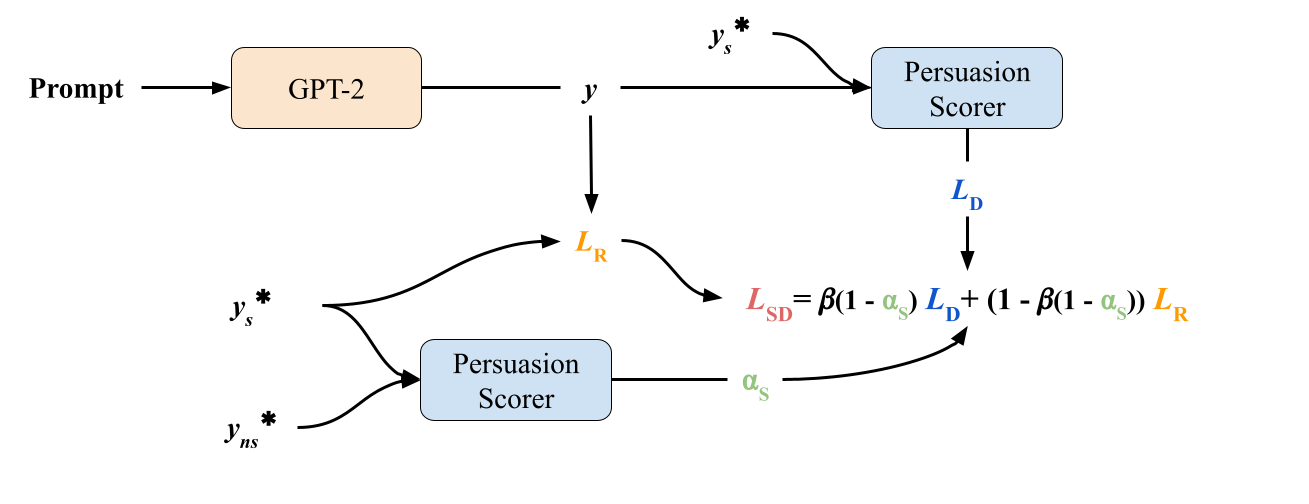
\includegraphics[width=0.9\linewidth]{figs/Architecture.png}
  \label{fig:architecture}
  \vspace{-5pt}
\end{figure*}

In this section, we infuse the stylistic preferences learned by our style discriminator in \Cref{sec_discriminator} into a GPT-2 model~\citep{radford2019language} pretrained on the causal language modeling (CLM) objective~\footnote{https://huggingface.co/gpt2}. The model takes in a textual prompt and generates text, $y$, that we want to infuse with the audience preferred style. For the persuasiveness task, the UKPConvArg1 dataset provides prompts for each argument pair. For the memorability task, we use the previous sentence as the prompt.

During training, we feed the prompt and feedback pair to GPT-2 - the more preferred (styled) sample, $y^*_s$, and the corresponding less-preferred (non-styled) sample, $y^*_{ns}$. We use an adversarial training paradigm to enable the generator to learn from the discriminator, illustrated in~\Cref{fig:architecture}. 

In~\Cref{subsec:si_training}, we introduce the custom loss function used for training. Then in~\Cref{subsec:si_dataset}, we discuss our augmentation approach for pairwise style data. Lastly, in~\Cref{subsec:si_gpt}, we describe GPT-2 and its benefits over other generation architectures.

\subsection{Training}
\label{subsec:si_training}

We utilize two losses during training: a reconstruction loss, $L_R$, and a discriminator loss, $L_D$. The reconstruction loss maximizes the log probability of the styled argument, $y_s^*$.

\begin{equation}
    L_{R} = -\frac{1}{N} \sum_{i=1}^{N} \log p(y_s^{*(i)})
\end{equation}

The reconstruction loss teaches the model to mimic the gold-standard samples. The discriminator loss maximizes the score of the discriminator, $\mathcal{D}$, and is formulated as:

\begin{equation}
    L_{D} = \mathcal{D}(y_s^*, y) - \frac{1}{N} \sum_{i=1}^{N} \hat{R}_i \log p(y^{(i)})
\end{equation}

where $y^{(i)}$ is the $i$-th token of the generated sentence $y$, and $\hat{R}_i$ is a baseline reward meant to reduce the noise from the discriminator. The baseline reward is meant to reduce the noise from the reward given by our discriminator \citep{ranzato2015sequence}. The baseline reward, $\hat{R}_i$, is calculated using a linear layer, with the input being the hidden states of our generator at timestep $i$. The intuition is that the linear layer approximates the value of the reward for a certain timestep and in practice, reduces the variance from the reward. We train the linear layer with the following loss:

\begin{equation}
    L_{BR} = \frac{1}{N} \sum_{i=1}^{N} |\mathcal{D}(y_s^*, y) - \hat{R}_i|^2
\end{equation}

where $\mathcal{D}(y_s^*, y)$ is the output of the discriminator when fed a gold argument and the generated argument (i.e. the reward). 

We find that too strong of a discriminator loss negatively impacts fluency. Thus, we introduce a regularization constant, $\beta$, to ensure that the discriminator loss remains only a fraction of the loss. The two losses are weighted together to create the final loss as follows:

\begin{equation}
    L_{SD} = C \cdot L_{D} + (1-C) \cdot L_{R}
\end{equation}

where $C = \beta (1-\alpha_{S})$ and $\alpha_{S} = \mathcal{D}(y_s^*, y_{ns}^*)$. Note that $y_{ns}^*$ is the non-styled training argument. 

Instead of making the weighted ratio between the two losses constant, we make them sample dependent. The intuition is that when $\alpha_{S}$ is high (e.g. the sample is persuasive), we can just use the reconstruction loss to replicate the gold standard which will directly reflect the style. However, when $\alpha_{S}$ is low (i.e. we have a weak sample), we instead switch to learning the trends from the discriminator. This loss is referred to as the sample-dependent discriminator (SD) loss. We also compare the discriminator loss with a simpler supervised loss defined as $L_{S} = \frac{1}{N} \sum_{i=1}^{N} \mathcal{D}(y_s^*, y^{(1..i)})$.

% \begin{equation}
%     L_{S} = \frac{1}{N} \sum_{i=1}^{N} \mathcal{D}(y_s^*, y^{(1..i)})
% \end{equation}

\subsection{Dataset Augmentation Approach}
\label{subsec:si_dataset}

The UKPConv1 and Cornell Movie Quotes corpora we presented in~\Cref{subsection:pairwise_datasets} provide approximately 16,000 and 2,200 unique pairs for stylistic feedback; not nearly enough to train a large language model. To increase our model's breadth of knowledge, we generate additional pairwise feedback with the CNN/Daily Mail dataset \citep{see-etal-2017-get}, containing over 300,000 unique news articles. 

First, we generate the Universal Sentence Embeddings~\citep{cer-2018} of all unique sentences in our style corpora (UKPConv1, Cornell) and external corpora (CNN/Daily Mail). For each candidate sentence in the external dataset, $s_i$, we find the top-k similar sentences ($y_1 ... y_k$) in the style corpus to be augmented. We then perform pairwise comparisons $\lor_{j} \mathcal{D}(s_i, y_j) > 0.5, j \in \{1, ..., k\}$ where if the discriminator prefers the candidate external sentence ($s_i$) over \textit{any one} of the similar sentences ($y_1 ... y_k$) from the style corpus, we include the pair. Through this bootstrapped augmentation method, we ensure we have sentences that are relatively more ``styled'', as defined by our discriminator, and similar to those in our existing corpus. 

\subsection{Style-Aware Generation with GPT-2}
\label{subsec:si_gpt}

The OpenAI GPT-2 \citep{radford2019language} model is a large transformer-based language model pretrained on nearly 8 million web pages, allowing generalization to many domains and tasks. This is closer to the unconstrained scenarios that we wish to target with our style-infusion task. Alternate generators such as pointer-generators rely on copying~\citep{xu2019clickbait}, thus introducing more limitations in the extent of style infusion. The ability to extensively pretrain transformer-based models makes them more widely applicable for syle infusion~\citep{gururangan2020pretraining}.

In this section, we introduced the adversarial training mechanism for the style-aware language generator and the bootstrapped data augmentation method used to produce robust generations. Next, we will introduce the baselines, evaluation metrics, and training settings.

% We found that the pre-trained GPT-2 provided by Huggingface ran into many issues with fluency and degeneration. Instead, we utilize GPT-2 fine-tuned on news data to provide an initial breadth of knowledge and diversity in generations. 